\documentclass[12pt]{article}
%\usepackage{fullpage}
\usepackage{epic}
\usepackage{eepic}
\usepackage{paralist}
\usepackage{graphicx}
\usepackage{algorithm,algorithmic}
\usepackage{tikz}
\usepackage{xcolor,colortbl}
\usepackage{amsmath, amssymb}

%%%%%%%%%%%%%%%%%%%%%%%%%%%%%%%%%%%%%%%%%%%%%%%%%%%%%%%%%%%%%%%%
% This is FULLPAGE.STY by H.Partl, Version 2 as of 15 Dec 1988.
% Document Style Option to fill the paper just like Plain TeX.

\typeout{Style Option FULLPAGE Version 2 as of 15 Dec 1988}

\topmargin 0pt
\advance \topmargin by -\headheight
\advance \topmargin by -\headsep

\textheight 8.9in

\oddsidemargin 0pt
\evensidemargin \oddsidemargin
\marginparwidth 0.5in

\textwidth 6.5in
%%%%%%%%%%%%%%%%%%%%%%%%%%%%%%%%%%%%%%%%%%%%%%%%%%%%%%%%%%%%%%%%

\pagestyle{empty}
\setlength{\oddsidemargin}{0in}
\setlength{\topmargin}{-0.8in}
\setlength{\textwidth}{6.8in}
\setlength{\textheight}{9.5in}

\setcounter{secnumdepth}{0}

\setlength{\parindent}{0in}
\addtolength{\parskip}{0.2cm}
\setlength{\fboxrule}{.5mm}\setlength{\fboxsep}{1.2mm}
\newlength{\boxlength}\setlength{\boxlength}{\textwidth}
\addtolength{\boxlength}{-4mm}

\newcommand{\algosolutionbox}[2]{
  \begin{center}
    \framebox{\parbox{\boxlength}{
        \textbf{CS 5722, Fall 2014} \hfill \textbf{#1}\\
        #2
      }}
  \end{center}}

\begin{document}

\algosolutionbox{Homework 6}{
  % TODO: fill in your own name, netID, and collaborators
  Group: Michael Jalkio, Kevin Li, Daniel Sperling\\
  NetIDs: mrj77, kyl27, dhs252
}

\section{1}
\subsection{a)}

Below follows a table demonstrating a solution with 17 channels:\\

\begin{table}[h]
\begin{tabular}{|r|l|l|l|l|l|l|l|l|l|l|l|l|l|l|l|l|l|}
\hline
\multicolumn{1}{|l|}{\textbf{}} & \multicolumn{17}{c|}{\textbf{Channels}}                                                                                                   \\ \hline
1                               & 0          & 0 & \textbf{1} & 0 & 0 & 0          & 0 & 0          & 0 & 0          & 0 & 0          & 0 & 0 & 0          & 0 & 0          \\ \cline{2-18} 
2                               & 0          & 0 & \textbf{1} & 0 & 0 & 0          & 0 & \textbf{1} & 0 & 0          & 0 & 0          & 0 & 0 & 0          & 0 & 0          \\ \cline{2-18} 
3                               & 0          & 0 & 0          & 0 & 0 & 0          & 0 & 0          & 0 & \textbf{1} & 0 & 0          & 0 & 0 & \textbf{1} & 0 & 0          \\ \cline{2-18} 
Cells  4                        & 0          & 0 & 0          & 0 & 0 & 0          & 0 & 0          & 0 & 0          & 0 & 0          & 0 & 0 & \textbf{1} & 0 & 0          \\ \cline{2-18} 
5                               & 0          & 0 & \textbf{1} & 0 & 0 & 0          & 0 & \textbf{1} & 0 & 0          & 0 & 0          & 0 & 0 & 0          & 0 & 0          \\ \cline{2-18} 
6                               & 0          & 0 & 0          & 0 & 0 & 0          & 0 & 0          & 0 & \textbf{1} & 0 & 0          & 0 & 0 & \textbf{1} & 0 & 0          \\ \cline{2-18} 
7                               & \textbf{1} & 0 & 0          & 0 & 0 & \textbf{1} & 0 & 0          & 0 & 0          & 0 & \textbf{1} & 0 & 0 & 0          & 0 & \textbf{1} \\ \hline
\end{tabular}
\end{table}

\subsection{b)}
Cell 1 has a conflict with 6, 2 with itself and 7, 3 with itself and 7, 4 with 5, 5 with itself and 6, 6 with 7 twice, and 7 with itself twice. This totals to the number of conflicts (the objective function) equaling \textbf{11 conflicts}.

\subsection{c)}
There are $7 * 13 = 91$ decision variables in such a problem.

\subsection{d)}
Yes, the minimum is 17. Each of the four channels in 7 must be separated by a minimum of four channels - this is 16 channels. There are then four assignments (two in 2 and two in 3, at least), that each must be at least two apart from  each other and two away from 7. It is impossible to assign all four of these in the three gaps of size four - only one assignment can go into each of those gaps. As such, at least one of those gaps must be widened by one - this is the 17th channel. As seen in part a, it is possible to do an assignment with 17 channels, so the minimum is 17.

\newpage
\section{2}
\subsection{i.}
Surface graph:\\
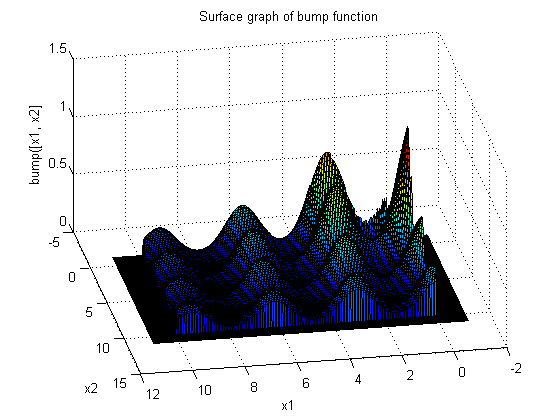
\includegraphics[height=10cm]{surface.png}

Contour graph:\\
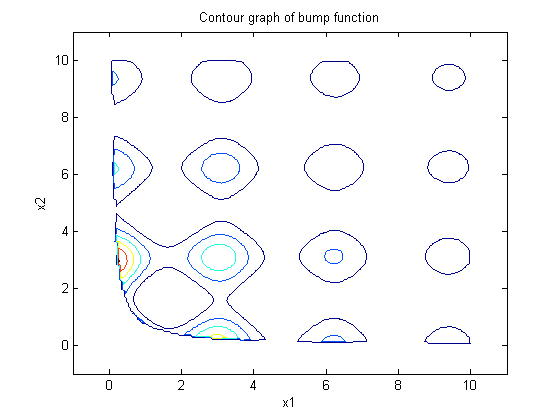
\includegraphics[height=10cm]{contour.png}

\subsection{ii.}
See attached code.

\subsection{iii.}
We chose to use a brute force ``experiment'' to find the best parameters.  We attempted all combinations of a large number of values for pMutation, pCrossover, and $V$.  For pMutation and pCrossover the values I tried were $[0.1, 0.2, 0.3, 0.4, 0.5, 0.6, 0.7, 0.8, 0.9]$ and for $V$ the values used were $[1.0, 2.0, 3.0, 4.0, 5.0, 6.0, 7.0, 8.0, 9.0, 10.0]$.  This took a long time to run.

For every combination we ran the genetic algorithm with 3 different initial populations (these were the same 3 for every trial), and then found the average elite bump function value.  We found that the combination of parameters with the highest average elite solution was $V=2.0$, $\text{pCrossover} =0.7$, and $\text{pMutation} =0.1$.

\subsection{iv.}
The average fitness of the fittest members of the population was $0.713401420075$.  The standard deviation of the fittest members of the population was $0.029858775518$.  The most fit member overall was:
\begin{align*} 
[3.064198856410788, 3.045933757913558, 3.0890092039978754, 3.073307537865654,\\ 2.858687419720218, 3.1461361256283227, 2.9391049363260886, 2.9330114316619595,\\ 2.9671806260328584, 0.4104508863181406, 0.39050790783291395, 0.49497721875386846,\\ 0.30254155872490707, 0.5434266329774524, 0.45720003735193226, 0.5109670303882086, \\ 0.46143215389831327, 0.5951647847564943, 0.3188694696960166, 0.2766059603205482]
\end{align*}
and it had a value of $0.758511263377$.  The least fit member overall was
\begin{align*}
[0.23600114763555305, 3.073816196073199, 2.9982296511970827, 3.202720680187456, \\ 2.9790205461501564, 3.022382774230237, 2.9139448909249692, 2.962096586726405, \\ 0.39667140927739053, 2.9372073655011506, 3.107027601546546, 3.026677239579595, \\ 1.3551503841351584, 0.8043543265228381, 0.4950037102453887, 0.4471412754809059, \\ 0.13667890818517237, 0.24682261227206115, 0.1630153732730799, 0.09618401485986772]
\end{align*}
and it had a value of $0.6401625568607917$.

Our plot appears in question 3.

\subsection{v.}
We feel that the arithmetic operator crossover could be good for this problem.  This is because of the nature of the bump function.  It takes the sum and the product of multiple numbers, so it's mostly about how those values interact together.  Because of this, it makes sense to take the average (so set $w=0.5$) of our two parents.  Doing this means that numbers that ``played nicely'' and led to good results will continue to contribute to their children with the same proportions.

\section{3}
\subsection{(a)}
See attached code.

\subsection{(b)}
The average fitness of the fittest members of the population was $0.568334178336$.  The standard deviation of the fittest members of the population was $0.0493294451417$.  The most fit member overall was:
\begin{align*} 
[3.2192452719665274, 3.1752263810653747, 3.3391066790724357, 3.0699177077612285,\\ 3.2767720905604634, 0.44277532656624796, 3.040299782122242, 3.2914751565371816,\\ 3.3073830752841777, 2.8941620504517847, 2.20417127826211, 0.25248928510518076,\\ 0.4174249174304465, 0.5029422220182223, 0.05775107009324282, 0.30699893367216624,\\ 0.4748142394786834, 0.36139033193565867, 0.36031050287714694, 0.7728398171231345]
\end{align*}
and it had a value of $0.6581828010261798$.  The least fit member overall was
\begin{align*}
[2.403178454838199, 0.33434678016001496, 3.111555871678033, 3.332531462978563,\\ 4.656845412954224, 3.41922063881561, 2.99654482242923, 0.3360796847780704,\\ 0.9428552414215912, 3.3022903545666082, 0.5311193521156884, 0.19765493674257806,\\ 2.4414923972041658, 0.2738397544478779, 0.08654813985261467, 2.7958082492484344,\\ 0.3913211802708072, 0.8773211370251517, 0.22628537805110427, 2.1291493186450428]
\end{align*}
and it had a value of $0.4742430215469693$.

\pagebreak
Graph for problems two and three:\\\\
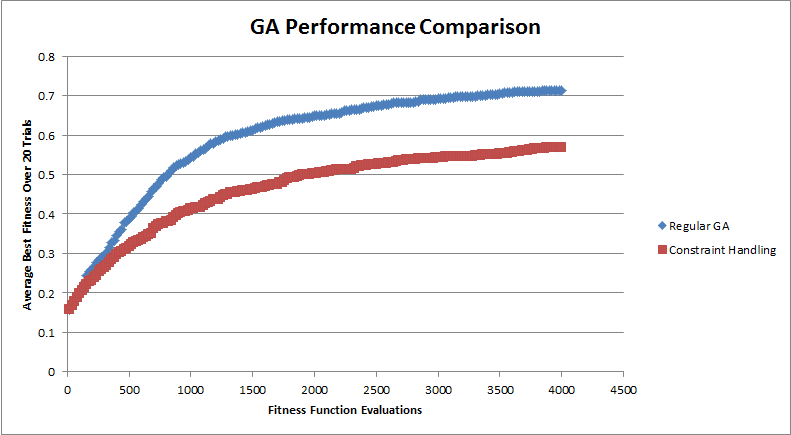
\includegraphics{ga_performance_graph.png}

\subsection{(c)}
The constraint handling techinique proposed by Deb (2000) reduced the performance of the genetic algorithm. The bump function returns $f_{min}$ - error if the solution is infeasible. This value may be positive, if the error is small and the current worst fitness is still large. Thus, an infeasible solution may be (incorrectly) assigned a positive fitness value.

\end{document}